\documentclass[11pt]{article}
\usepackage[margin=1in]{geometry}
\usepackage{amsmath,amssymb,amsthm,mathtools}
\usepackage{dsfont}
\usepackage{graphicx}
\usepackage{booktabs}
\usepackage{array}
\usepackage{placeins}
\usepackage[hyphens]{url}
\usepackage{microtype}
\usepackage{xcolor}
\usepackage{tikz}
\usepackage{caption}
\usepackage{subcaption}
\usepackage[colorlinks=true,linkcolor=blue!55!black,citecolor=blue!55!black,urlcolor=blue!55!black]{hyperref}

\newcommand{\Tr}{\operatorname{Tr}}
\newcommand{\PB}{P_{\mathrm B}}
\newcommand{\Var}{\operatorname{Var}}
\newcommand{\Np}{N'}
\newcommand{\one}{\mathds 1}
\newcommand{\End}{\operatorname{End}}
\newcommand{\Ad}{\operatorname{Ad}}

% status tags
\definecolor{cest}{RGB}{30,90,160}
\definecolor{cder}{RGB}{20,120,70}
\definecolor{cnum}{RGB}{150,90,10}
\definecolor{cconj}{RGB}{160,40,40}
\newcommand{\tagbox}[2]{\textsf{\small\color{#1}[#2]}}
\newcommand{\EST}{\tagbox{cest}{literature}}
\newcommand{\DER}{\tagbox{cder}{derived}}
\newcommand{\VER}{\tagbox{cder}{derived + verified}}
\newcommand{\NUM}{\tagbox{cnum}{numerical}}
\newcommand{\CONJ}{\tagbox{cconj}{conjecture}}
\newcommand{\INTERP}{\tagbox{cconj}{interpretation}}

% chord-diagram palette (matches the data figures)
\definecolor{cP}{HTML}{2A78D6}   % P arcs (BPS projector)
\definecolor{cPp}{HTML}{EB6834}  % P' = U P U arcs
\definecolor{cX}{HTML}{8E2C8A}   % chords joining P and P' arcs: weight x
\definecolor{cP2}{HTML}{1BAF7A}  % an independent second model
\tikzset{
  Parc/.style={line width=3.4pt, cP},
  Pparc/.style={line width=3.4pt, cPp},
  Ptwo/.style={line width=3.4pt, cP2},
  triv/.style={line width=1.3pt, gray!65, dash pattern=on 2.2pt off 1.6pt},
  chP/.style={line width=1.0pt, cP!85!black},
  chPp/.style={line width=1.0pt, cPp!90!black},
  chPtwo/.style={line width=1.0pt, cP2!85!black},
  chX/.style={line width=1.15pt, cX, dash pattern=on 3.2pt off 1.8pt},
  Umark/.style={draw=black, fill=white, rectangle, inner sep=1.8pt, line width=0.8pt},
}
% \chord[style]{angle1}{angle2}{radius}: a chord bowing towards the centre
\newcommand{\chord}[4][]{\draw[#1] ({#2}:{#4}) .. controls ({#2}:{0.32*#4}) and ({#3}:{0.32*#4}) .. ({#3}:{#4});}
\newcommand{\Umk}[2]{\node[Umark] at ({#1}:{#2}) {};}

\newtheorem{proposition}{Proposition}
\theoremstyle{remark}
\newtheorem*{remark}{Remark}

\title{\bf Progress report, 29 September 2026:\\ the decoder's moments from operator size ---\\
exact sum rules, two correlated BPS spaces,\\ and chord pictures toward a gravity dual}
\author{\texttt{syk\_gravity} project\\[2pt]\small Drafted by Claude for J.~Chryssanthacopoulos; code state: commit \texttt{774934a} + working tree}
\date{}

\emergencystretch=2em
\begin{document}
\maketitle

\begin{abstract}
\noindent
Yesterday's checkpoint showed that the variance of the uplift decoder $O=P(1-n_i)P$ of one-flavor $\mathcal N{=}2$
SYK is reproduced to about 2\,\% by the finite-$\lambda$ super-chord theory. It also showed that, in that theory, the
Haar/Wachter value is exactly the contribution of the zero-length supersymmetric wormhole. This report takes the
next steps. It keeps only results that survived a claim-by-claim audit of the working note.

\begin{itemize}\itemsep1pt
\item \textbf{Two correlated BPS spaces.} The decoder spectrum is the principal-angle law between the BPS space $B$
  and $B'=UB$, where $U=(-1)^{n_i}$. $B'$ is the BPS space of the same model with the new mode's couplings reversed.
  In chord language the zero-temperature boundary splits into $P$- and $P'$-arcs, and chords joining the two
  kinds carry a weight $x$.
\item \textbf{The variance is operator size.} The SYK coupling ensemble is $U(N)$-invariant. As a result, the
  decoder variance is an \emph{exact finite-$N$ functional of the operator-size spectrum $w_k$ of the BPS
  projector}:
  \[
  r=1-\frac{4\,\langle k(N+1-k)\rangle_w}{N(N+1)}\quad\text{(half filling)},\qquad w_0=a\ \text{exactly}.
  \]
  This is the exact counterpart of the wormhole identity: the identity (size-0) component of $P$ plays the
  zero-length wormhole. It reproduces SYK to 0.1--0.8\,\%.
\item \textbf{Freeness is flat transmission.} Two independent SYK BPS spaces are \emph{not} free relative to each
  other. Their fourth moment is predicted exactly from single-model size data, and the prediction matches pair
  measurements to 0.01--0.2\,\%.
\item \textbf{The fourth moment.} The decoder's $T_4$ splits exactly into a part fixed by the variance, a part fixed
  by the size spectrum, and a four-point remainder $R$ ($\approx21\%$ of the excess at $N'=13$--14), which remains
  open.
\end{itemize}
The exact identities are kinematics (representation theory of $U(N)$). The dynamics, and hence any gravity dual,
enters only through the size spectrum and its multi-copy generalizations. Tags: \DER, \VER, \NUM, \INTERP, \CONJ.
\end{abstract}

\tableofcontents

%=====================================================================
\section{Summary of results}
%=====================================================================
\begin{enumerate}\itemsep3pt
\item \VER\ \textbf{Parity form.} $1-n_i=\frac12(1+U)$, $U=(-1)^{n_i}$, so the decoder is $\frac12(1+PUP)$. With
  $P'=UPU$, $(PUP)^2=PP'P$. $P'$ is the BPS projector of $Q'=UQU$: the same supercharge with every coupling containing
  mode $i$ sign-flipped (\S\ref{sec:parity}).
\item \DER\ \textbf{Z$_2$ chord rule.} A $Q$-chord whose endpoints are separated by an odd number of $U$-insertions
  picks up $(-1)^{[i\in I]}$, i.e.\ weight $x$ on average. Chords joining arcs of the same kind get 1. This is exact
  per chord; independence between chords is the double-scaled approximation (\S\ref{sec:chords},
  Fig.~\ref{fig:arcs2}--\ref{fig:arcs4}).
\item \NUM\ \textbf{Tuning $x$ at fixed $P$.} Parity projectors on $s$ modes tune $x$ from $0.57$ ($s=1$, the
  decoder) to exactly $0$ ($s=\Np/2$).
  \begin{itemize}\itemsep1pt
  \item The second moment becomes free ($r\to a$).
  \item The fourth and sixth moments do not ($+5.6\%$, $+10\%$ at $\Np=14$, growing with $\Np$)
    (\S\ref{sec:family}).
  \end{itemize}
\item \VER\ \textbf{Exact variance sum rule.}
  \begin{itemize}\itemsep1pt
  \item $E[P]=a\one$, and $E[T_2]=\sum_kw_k\hat\chi_k(U)$, with $w_0=a$ exactly.
  \item For the single-mode decoder, $\hat\chi_k=1-4k(N+1-k)/(N(N+1))$, which gives the boxed formula above.
  \item It agrees with the SYK campaign to 0.1--0.8\,\% for $\Np=8\ldots14$ (\S\ref{sec:size}).
  \end{itemize}
\item \VER\ \textbf{Only even sizes at half filling.} Odd-size weights are $\le2\times10^{-28}$, i.e.\ exactly zero.
  A particle--hole argument (sketch) explains it; the same symmetry gives the known $\lambda\leftrightarrow1-\lambda$
  pairing.
\item \NUM\ \textbf{Size $\leftrightarrow$ wormhole length (empirical).} $w_{2n}$ tracks the super-chord
  wormhole-length distribution $P_n$ to 10--20\,\%, and the characters track the matter weights $x^{2n}$
  (\S\ref{sec:chordcomp}).
\item \VER\ \textbf{Transmission.}
  \begin{itemize}\itemsep1pt
  \item $X\mapsto E[PXP]$ acts on size-$k$ operators as a scalar $\phi_k$, which is a universal linear function of
    $w$.
  \item Haar: $\phi_{k\ge1}=a^2$ (flat). SYK: $\phi_k>a^2$ at small $k$.
  \item Two independent models: $E\,\tau(P_1P_2P_1P_2)=\sum_k\phi_kw_k$, exactly. SYK is $+0.6$, $+2.0$, $+4.3\%$
    above free at $\Np=10,12,14$, and the prediction matches measurement to $\le0.2\%$ (\S\ref{sec:transmission}).
  \end{itemize}
\item \VER\ \textbf{Decoder fourth moment.} $T_4=a^2+2a(T_2-a)+S+R$ exactly, with $S=\sum_{k\ge1}\phi_kw_k$. At
  $\Np=13$--14, 74\,\% / 5\,\% / 21\,\% of the excess over free come from the variance term, the size-spectrum term
  and the remainder $R$ (\S\ref{sec:T4}).
\item \DER\ \textbf{Correction to yesterday's conjecture.} ``The free law is the zero-length truncation'' holds for
  $m_2$ only. Already for Haar $P$, the free $T_4$ receives $a^2(1-a)$ from nonzero sizes. The correct
  characterization is: \emph{freeness = flat transmission}.
\end{enumerate}

%=====================================================================
\section{Setup and recap}\label{sec:setup}
%=====================================================================
\paragraph{Model and decoder.}
One-flavor $\mathcal N{=}2$ SYK on $\Np$ complex fermions with $Q=\sum_{|I|=p}C_I\psi_I$ ($p=3$) and i.i.d.\ complex
Gaussian couplings; $H=\{Q,Q^\dagger\}$.
\begin{itemize}\itemsep1pt
\item Fermion-number sector $F=\lfloor\Np/2\rfloor$ (half filling at even $\Np$), the Fock space $\Lambda^F$ of dimension
  $D=\binom{\Np}{F}$. $B\subset\Lambda^F$ is the BPS space, $d=\dim B$, $a=d/D$. $P$ always denotes the BPS projector,
  and $\tau=\Tr_B/d$. In \S\S\ref{sec:size}--\ref{sec:transmission} and Appendix~A we write $N\equiv\Np$.
  (The code and earlier notes call the sector $P$.)
\item Decoder: $O=P\Pi P$ with $\Pi=1-n_i$ ($i$ the new mode; all modes are equivalent in distribution).
  Eigenvalues $\lambda\in[0,1]$; $b=1-F/\Np$.
\item Rigidity: $r=\Var(\lambda)/[b(1-b)]$. Haar/Wachter predicts $r=a$.
\end{itemize}

\paragraph{Yesterday's result \NUM\ + \EST.} The Boruch--Lin--Yan (BLY)~\cite{BLY} double-scaled two-point function,
with $\lambda=2p^2/\Np$ and $\Delta=1/p$, gives $r=\sum_nP_nx^{2n}$. Here $P_n$ is the chord-number (wormhole-length)
distribution of the supersymmetric Hartle--Hawking state, $x=q^{\Delta}$, and $P_0=a_\lambda$ is the double-scaled BPS
fraction. It matches SYK to $\approx2\%$. The Haar value is the $n=0$ term. That identity was exact only within the
double-scaled theory, and $a_\lambda$ exceeds the exact $a$ by 2--8\,\% at $\Np=8$--14 (Table~\ref{tab:chordcomp}). Section~\ref{sec:size} removes both
limitations.

%=====================================================================
\section{The decoder as the overlap of two correlated BPS spaces}\label{sec:parity}
%=====================================================================
\subsection{Parity form \VER}
Since $n_i$ is a projector, $\Pi=1-n_i=\frac12(1+U)$ with $U=(-1)^{n_i}$, a unitary involution. So
$P\Pi P=\frac12(P+PUP)$, and on $B$
\begin{equation}
\lambda=\tfrac12(1+\mu),\qquad \mu\in\mathrm{spec}(PUP|_B)\subset[-1,1],\qquad
T_m\equiv\tau\big((PUP)^m\big)=E[\mu^m] .
\end{equation}
Using $U^2=1$,
\begin{equation}
(PUP)^2=P\,(UPU)\,P=P\,P'\,P,\qquad P'\equiv UPU .
\label{eq:PPp}
\end{equation}
$P'$ is the BPS projector of $Q'=UQU=\sum_I(-1)^{[i\in I]}C_I\psi_I$, the model with all couplings involving mode $i$
reversed. Hence $\mu^2$ are the squared cosines of the principal angles between $B$ and $B'=UB$. In uplift language
(Chryssanthacopoulos--Vegh~\cite{CV}): writing a BPS state as $\Psi=a+b\wedge e_i$, one has
$\langle\Psi|U\Psi\rangle=\|a\|^2-\|b\|^2=2\lambda-1$. So the decoder measures how much the BPS space rotates when the
new mode's couplings are reversed. At half filling the spectrum is symmetric ($T_{\rm odd}=0$, verified to
$10^{-16}$; \S\ref{sec:even}), so the principal-angle law determines the decoder law completely.

\subsection{Chord picture: arcs and the Z$_2$ rule \DER}\label{sec:chords}
For a supercharge term, $U\psi_IU=(-1)^{[i\in I]}\psi_I$. In a trace of a $Q,Q^\dagger$ word with an \emph{even}
number $m$ of $U$ insertions, move all $U$'s together ($U^m=1$). Each supercharge factor picks up
$(-1)^{[i\in I]}$ once for every $U$ it passes. A $Q$-chord (a Wick pair $C_IC_I^*$) therefore carries
$(-1)^{[i\in I]\cdot\#}$, where $\#$ is the number of $U$'s separating its endpoints. Averaged over its random index
set $I$:
\begin{equation}
\text{weight}=\begin{cases}x, & \#\ \text{odd}\\ 1,&\#\ \text{even}\end{cases},\quad
x=1-\frac{2p}{\Np}\ \text{(exact, per chord)},\quad x\simeq e^{-2p/\Np}=q^{1/p}\ \ \text{(double-scaled)},
\end{equation}
since $i\in I$ with probability $p/\Np$; here $q=e^{-\lambda}$, $\lambda=2p^2/\Np$.
Label the $m$ zero-temperature arcs alternately $P$ and $P'$. A chord joining a $P$-arc to a $P'$-arc gets $x$; a
chord joining arcs of the same kind gets 1. Figure~\ref{fig:arcs2} shows $m=2$, which reproduces BLY's horizontal
matter chord and $r=\sum_nP_nx^{2n}$. Figure~\ref{fig:arcs4} shows $m=4$. There a chord spanning two opposite $P$-arcs
gets weight 1, not $x^2$, so the higher moments are \emph{not} given by the Gaussian-matter (q-Gaussian) rule. That
the per-chord averages multiply is the double-scaled approximation: at finite $N$, different chords share site
indices.

\begin{figure}[t]
\centering
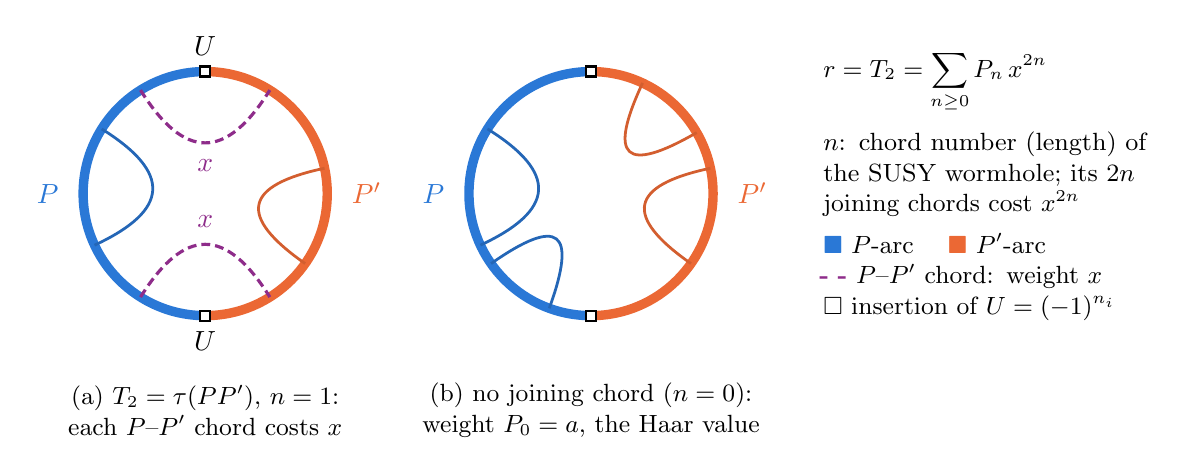
\begin{tikzpicture}
\def\R{1.55}
\begin{scope}
  \draw[Parc] (90:\R) arc[start angle=90, end angle=270, radius=\R];
  \draw[Pparc] (-90:\R) arc[start angle=-90, end angle=90, radius=\R];
  \chord[chP]{148}{205}{\R}
  \chord[chPp]{-35}{12}{\R}
  \chord[chX]{122}{58}{\R}
  \chord[chX]{238}{-58}{\R}
  \Umk{90}{\R}\Umk{270}{\R}
  \node at (90:\R+0.32) {$U$}; \node at (270:\R+0.32) {$U$};
  \node[cP] at (180:\R+0.45) {$P$}; \node[cPp] at (0:\R+0.5) {$P'$};
  \node[cX] at (0,0.36) {$x$}; \node[cX] at (0,-0.36) {$x$};
  \node[align=center, font=\small] at (0,-2.75) {(a) $T_2=\tau(PP')$, $n=1$:\\ each $P$--$P'$ chord costs $x$};
\end{scope}
\begin{scope}[xshift=4.9cm]
  \draw[Parc] (90:\R) arc[start angle=90, end angle=270, radius=\R];
  \draw[Pparc] (-90:\R) arc[start angle=-90, end angle=90, radius=\R];
  \chord[chP]{148}{205}{\R}
  \chord[chP]{215}{250}{\R}
  \chord[chPp]{-35}{12}{\R}
  \chord[chPp]{30}{65}{\R}
  \Umk{90}{\R}\Umk{270}{\R}
  \node[cP] at (180:\R+0.45) {$P$}; \node[cPp] at (0:\R+0.5) {$P'$};
  \node[align=center, font=\small] at (0,-2.75) {(b) no joining chord ($n=0$):\\ weight $P_0=a$, the Haar value};
\end{scope}
\begin{scope}[xshift=10.0cm]
  \node[align=left, font=\small, text width=4.3cm] at (0,0.1) {
  $\displaystyle r=T_2=\sum_{n\ge0}P_n\,x^{2n}$\\[6pt]
  $n$: chord number (length) of the SUSY wormhole; its $2n$ joining chords cost $x^{2n}$\\[4pt]
  \textcolor{cP}{$\blacksquare$}~$P$-arc \quad \textcolor{cPp}{$\blacksquare$}~$P'$-arc\\
  \textcolor{cX}{\bf - -}~$P$--$P'$ chord: weight $x$\\
  $\square$~insertion of $U=(-1)^{n_i}$};
\end{scope}
\end{tikzpicture}
\caption{\DER\ The second moment as a two-arc chord diagram at zero temperature. The two $U$ insertions split the
boundary into a $P$-arc and a $P'$-arc. Chords with both ends on one arc cost 1. Chords joining the arcs cost $x$
each. Summing over diagrams gives $\sum_nP_nx^{2n}$ (BLY eqs.~4.5--4.8, with yesterday's identification
$\lambda=2p^2/\Np$, $\Delta=1/p$). The $n=0$ class (b)
is the zero-length wormhole, whose weight $P_0$ is the BPS fraction, i.e.\ the free value.}
\label{fig:arcs2}
\end{figure}

\begin{figure}[t]
\centering
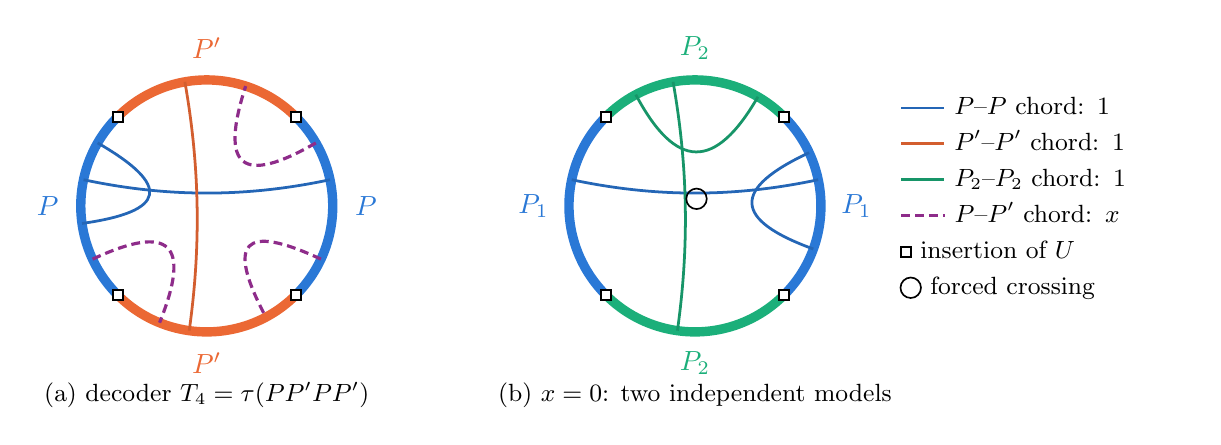
\begin{tikzpicture}
\def\R{1.6}
\begin{scope}
  \draw[Parc] (-45:\R) arc[start angle=-45, end angle=45, radius=\R];
  \draw[Pparc] (45:\R) arc[start angle=45, end angle=135, radius=\R];
  \draw[Parc] (135:\R) arc[start angle=135, end angle=225, radius=\R];
  \draw[Pparc] (225:\R) arc[start angle=225, end angle=315, radius=\R];
  \chord[chP]{12}{168}{\R}
  \chord[chPp]{100}{262}{\R}
  \chord[chX]{30}{72}{\R}
  \chord[chX]{205}{248}{\R}
  \chord[chX]{-25}{-62}{\R}
  \chord[chP]{150}{188}{\R}
  \Umk{45}{\R}\Umk{135}{\R}\Umk{225}{\R}\Umk{315}{\R}
  \node[cP] at (0:\R+0.42) {$P$}; \node[cP] at (180:\R+0.42) {$P$};
  \node[cPp] at (90:\R+0.4) {$P'$}; \node[cPp] at (270:\R+0.4) {$P'$};
  \node[align=center, font=\small] at (0,-2.4) {(a) decoder $T_4=\tau(PP'PP')$};
\end{scope}
\begin{scope}[xshift=6.2cm]
  \draw[Parc] (-45:\R) arc[start angle=-45, end angle=45, radius=\R];
  \draw[Ptwo] (45:\R) arc[start angle=45, end angle=135, radius=\R];
  \draw[Parc] (135:\R) arc[start angle=135, end angle=225, radius=\R];
  \draw[Ptwo] (225:\R) arc[start angle=225, end angle=315, radius=\R];
  \chord[chP]{12}{168}{\R}
  \chord[chPtwo]{100}{262}{\R}
  \chord[chP]{-20}{25}{\R}
  \chord[chPtwo]{60}{118}{\R}
  \Umk{45}{\R}\Umk{135}{\R}\Umk{225}{\R}\Umk{315}{\R}
  \node[cP] at (0:\R+0.45) {$P_1$}; \node[cP] at (180:\R+0.45) {$P_1$};
  \node[cP2] at (90:\R+0.4) {$P_2$}; \node[cP2] at (270:\R+0.4) {$P_2$};
  \draw[black, line width=0.6pt] (0.02,0.09) circle (0.13);
  \node[align=center, font=\small] at (0,-2.4) {(b) $x=0$: two independent models};
\end{scope}
\begin{scope}[xshift=10.6cm]
  \node[align=left, font=\small, text width=3.6cm] at (0,0.1) {
  \tikz[baseline=-0.6ex]\draw[chP](0,0)--(0.55,0);~$P$--$P$ chord: 1\\[2pt]
  \tikz[baseline=-0.6ex]\draw[chPp](0,0)--(0.55,0);~$P'$--$P'$ chord: 1\\[2pt]
  \tikz[baseline=-0.6ex]\draw[chPtwo](0,0)--(0.55,0);~$P_2$--$P_2$ chord: 1\\[2pt]
  \tikz[baseline=-0.6ex]\draw[chX](0,0)--(0.55,0);~$P$--$P'$ chord: $x$\\[2pt]
  \tikz[baseline=-0.6ex]\node[Umark]{};~insertion of $U$\\[2pt]
  \tikz[baseline=-0.6ex]\draw[line width=0.6pt](0,0) circle (0.13);~forced crossing};
\end{scope}
\end{tikzpicture}
\caption{\DER\ + \INTERP\ Four arcs. (a) The decoder's fourth moment $T_4=\tau(PP'PP')$. A chord spanning the two
$P$-arcs (or the two $P'$-arcs) separates an even number of $U$'s and costs 1, not $x^2$: the Z$_2$ rule differs from
Gaussian matter. (b) At $x=0$ only same-kind chords survive, as for two independent SYK models. The two ``across''
chords must then cross (circled), and their crossing weight comes from shared site indices. If such crossings were
forbidden (crossing weight 0, as for freely independent $q$-Gaussians), the two BPS spaces would be free. In SYK they
are not: $E\,\tau(P_1P_2P_1P_2)-T_4^{\rm free}=\sum_{k\ge1}\delta\phi_k\,w_k>0$ (\S\ref{sec:transmission}).}
\label{fig:arcs4}
\end{figure}

\subsection{Tuning $x$ at fixed BPS space: the parity family \NUM}\label{sec:family}
Replace $U$ by $U_S=(-1)^{N_S}$ with $|S|=s$ and $S\ni i$. Then $U_S\psi_IU_S=(-1)^{|I\cap S|}\psi_I$, and
\begin{equation}
x_s=\sum_k(-1)^k\binom sk\binom{\Np-s}{p-k}\Big/\binom{\Np}{p}\qquad(\text{exact per chord}).
\end{equation}
For odd $p$, $|I\cap S^c|=p-|I\cap S|$ gives $x_{\Np-s}=-x_s$, so $x=0$ \emph{exactly} at $s=\Np/2$. (With the
charge fixed, $U_{S^c}=\pm U_S$ is the same probe.) The
BPS projector is the same for every $s$; only the probe changes. Figure~\ref{fig:family} and
Table~\ref{tab:family} give the results.

\begin{figure}[t]
\centering
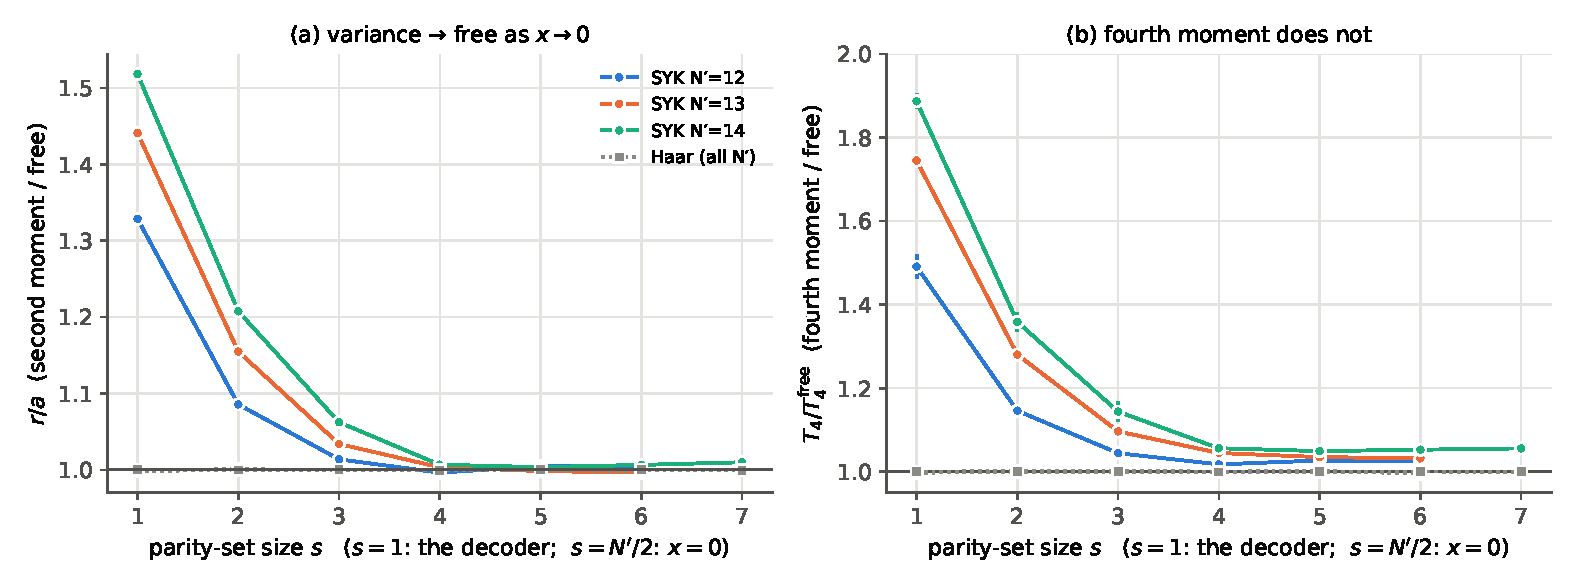
\includegraphics[width=\textwidth]{progress_2026-09-29_figs/fig_parity_family.pdf}
\caption{\NUM\ Parity family at $\Np=12,13,14$ (4 SYK realizations each; Haar controls dotted). Exact per-chord weights
at $\Np=14$: $x_s=0.571,0.275,0.088,-0.011,-0.044,-0.033,0$ for $s=1\ldots7$. (a) The rigidity $r/a$ returns to the free
value as $x\to0$. (b) The fourth moment does not: an $x$-independent excess remains. The free baseline is the
Wachter$(a,b)$ law (with $b\neq\frac12$ at odd $\Np$).}
\label{fig:family}
\end{figure}

\begin{table}[h]
\centering\small
\begin{tabular}{@{}lccccccc@{}}
\toprule
& \multicolumn{5}{c}{$\Np=14$, 4 realizations} & \multicolumn{2}{c}{$x\approx0$ across sizes}\\
\cmidrule(lr){2-6}\cmidrule(l){7-8}
$s$ & $x_s$ & $r/a$ & $T_4/T_4^{\rm free}$ & $T_6/T_6^{\rm free}$ & KS to Wachter & $\Np$ & $T_4/T_4^{\rm free}$ at $s=\lfloor \Np/2\rfloor$\\
\midrule
1 (decoder) & $+0.571$ & 1.518 & $1.887\pm0.018$ & 2.21 & 0.145 & 10 & $1.014\pm0.007$\\
2 & $+0.275$ & 1.208 & $1.359\pm0.024$ & 1.49 & 0.080 & 12 & $1.025\pm0.004$\\
3 & $+0.088$ & 1.062 & $1.144\pm0.024$ & 1.22 & 0.035 & 13 & $1.032\pm0.010$\\
4 & $-0.011$ & 1.007 & $1.056\pm0.014$ & 1.11 & 0.026 & 14 & $1.056\pm0.002$\\
7 & 0 & 1.010 & $1.056\pm0.002$ & 1.10 & 0.021 & Haar & $1.000\pm0.001$\\
\bottomrule
\end{tabular}
\caption{\NUM\ Moments relative to free compression (Wachter$(a,b)$). The KS distance of Haar controls is 0.002.
$T_4^{\rm free}=2a^2-a^3$ and $T_6^{\rm free}=5a^3-6a^4+2a^5$ at $b=\frac12$ (free cumulants of a symmetric $\pm1$
variable: $\kappa_2=1$, $\kappa_4=-1$, $\kappa_6=2$).}
\label{tab:family}
\end{table}

\paragraph{Findings.}
\begin{itemize}\itemsep1pt
\item \textbf{The variance becomes free} as the matter weight is removed. The small residual at $x=0$
  ($r/a=1.010\pm0.002$ at $\Np=14$) is accounted for at the $2\sigma$ level by \S\ref{sec:size} (predicted 1.006).
\item \textbf{The fourth moment does not.} An $x$-independent excess remains and grows with $\Np$. Section
  \ref{sec:transmission} identifies its origin: two different SYK BPS spaces are not mutually free.
\end{itemize}

%=====================================================================
\section{Operator size of the BPS projector: an exact variance sum rule}\label{sec:size}
%=====================================================================
\subsection{$U(N)$ invariance \DER}
The couplings are i.i.d.\ standard complex Gaussians in the orthonormal basis $e_{i_1}\wedge\cdots\wedge e_{i_p}$ of
$\Lambda^p\mathbb C^N$. The induced action of $g\in U(N)$ (single-particle rotations) is unitary, so the coupling law is
$U(N)$-invariant. $Q=\omega\wedge$ and $Q^\dagger$ are covariant, so $P(g\omega)=\rho(g)P(\omega)\rho(g)^\dagger$ and the
BPS-projector ensemble is invariant under conjugation. Since $\Lambda^F$ is irreducible, Schur's lemma gives
\begin{equation}
E[P]=a\,\one\qquad\text{exactly.}
\end{equation}

\subsection{Size sectors \VER}
Under $U(N)$ conjugation, $\End(\Lambda^F)=\Lambda^F\otimes(\Lambda^F)^*$ decomposes multiplicity-free,
\begin{equation}
\End(\Lambda^F)=\bigoplus_{k=0}^{\min(F,N-F)}V_k,\qquad \dim V_k=\binom Nk^2-\binom N{k-1}^2 .
\end{equation}
Here $V_k$ consists of the traceless ``$k$-body'' operators (highest weight $(1^k,0,\ldots,0,(-1)^k)$), and the adjoint
Casimir $C(X)=\sum_{ab}[E_{ab},[E_{ba},X]]$, with $E_{ab}=\bar\psi_a\psi_b$, acts on $V_k$ as $2k(N+1-k)$. Write
$P=\sum_kP^{(k)}$ and define the \textbf{size spectrum}
\begin{equation}
w_k=\frac{\|P^{(k)}\|_F^2}{d},\qquad \sum_kw_k=1,\qquad \boxed{w_0=a\ \text{exactly, per realization}},
\end{equation}
since $P^{(0)}=(\Tr P/D)\one=a\one$. (Verified: full diagonalization of the Casimir superoperator at $N=6$
reproduces the spectrum, the multiplicities and the parity characters; the size components reconstruct $P$ with
residual $<10^{-10}$ at $N=8$; \path{tests/test_size_decomposition.py}.)

\subsection{The sum rule and its closed form for the decoder \VER}
Any $g\in U(N)$ preserves every $V_k$, so $\tau(PgPg^\dagger)=\frac1d\sum_k\langle P^{(k)},\Ad_gP^{(k)}\rangle$ with no
cross terms. By invariance, $E\big[|P^{(k)}\rangle\rangle\langle\langle P^{(k)}|\big]\propto\one_{V_k}$ (Schur), hence
\begin{equation}
E\big[\tau(PgPg^\dagger)\big]=\sum_kw_k\,\hat\chi_k(g),\qquad \hat\chi_k(g)=\frac{|\chi_{\Lambda^k}(g)|^2-|\chi_{\Lambda^{k-1}}(g)|^2}{\dim V_k}.
\label{eq:sumrule}
\end{equation}
Equation~\eqref{eq:sumrule} is exact at finite $N$, for any charge sector and any group element. For parities,
$\chi_{\Lambda^k}(U_S)$ is a Krawtchouk polynomial. For the decoder ($g=U$, a reflection), the character is a linear
function of the Casimir (Appendix~\ref{app:reflection}):
\begin{equation}
\hat\chi_k(U)=1-\frac{4k(N+1-k)}{N(N+1)}\quad\Longrightarrow\quad
\boxed{\;E[T_2]=1-\frac{4\,\langle k(N+1-k)\rangle_w}{N(N+1)}=a+\sum_{k\ge1}w_k\hat\chi_k(U)\;}
\label{eq:rsize}
\end{equation}
At half filling $E[T_2]=r$.
\begin{itemize}\itemsep1pt
\item \textbf{The decoder variance measures the mean operator size (adjoint Casimir) of the BPS projector.}
\item The identity component contributes exactly $a$, the Haar value. The deviation from freeness is $P$'s weight on
  nonzero sizes, weighted by the probe's characters.
\item \textbf{Haar check \DER.} For Haar $P$, $w_k=(1-a)\dim V_k/(D^2-1)$ ($k\ge1$). Since
  $\sum_k\dim V_k\hat\chi_k=|\Tr U|^2$, this gives $E[T_2]=(aD^2-1)/(D^2-1)$ at half filling, the exact Weingarten
  value.
\end{itemize}

\subsection{Only even sizes at half filling \VER\ (sketch)}\label{sec:even}
Particle--hole conjugation $V$ ($\psi\leftrightarrow\bar\psi$) maps $\Lambda^{N/2}$ to itself and $Q_\omega$ to
$Q_{\bar\omega}^\dagger$. Hence $VB(\omega)=B(\bar\omega)=\overline{B(\omega)}$, i.e.\ $VPV^\dagger=P^T$. The map
$X\mapsto(VXV^\dagger)^T$ acts on $V_k$ as $(-1)^k$, so $P^{(k)}=0$ for odd $k$. (Signs are not tracked in detail.
Numerically, odd weights are $\le2\times10^{-28}$ at $\Np=8$--14, and nonzero at odd $\Np$.) The same map sends
$n_i\mapsto1-n_i$, which gives $T_{\rm odd}=0$ and the pairing $\lambda\leftrightarrow1-\lambda$.

\subsection{SYK numbers \NUM}
Table~\ref{tab:sumrule} tests eq.~\eqref{eq:rsize} against the independent chord-invariant campaign of 28 September.
It has no free parameter: the size weights come from a separate set of realizations, and the characters are exact.
Figure~\ref{fig:size}a shows where the weight sits.
\begin{table}[h]
\centering\small
\begin{tabular}{@{}ccccccccc@{}}
\toprule
$\Np$ & $w_0\,(=a)$ & $w_2$ & $w_4$ & $w_6$ & $\langle k\rangle_w$ & $E[T_2]$, eq.~\eqref{eq:rsize} & SYK $T_2$ & diff.\\
\midrule
8 & 0.7714 & 0.2128 & 0.0158 & -- & 0.49 & 0.8170 & $0.8186\pm0.0008$ & $-0.2\%$\\
10 & 0.6429 & 0.2997 & 0.0574 & -- & 0.83 & 0.7454 & $0.7463\pm0.0007$ & $-0.1\%$\\
12 & 0.5260 & 0.3486 & 0.1119 & 0.0135 & 1.23 & 0.6855 & $0.6874\pm0.0009$ & $-0.3\%$\\
13$^\ast$ & 0.4248 & 0.3398 & 0.1435 & 0.0318 & 1.64 & 0.6176 & $0.6193\pm0.0018$ & $-0.3\%$\\
14 & 0.4248 & 0.3706 & 0.1629 & 0.0416 & 1.64 & 0.6371 & $0.6420\pm0.0037$ & $-0.8\%$\\
\midrule
14, Haar & 0.4248 & 0.0004 & 0.0425 & 0.2448 & 3.33 & 0.4248 & $0.4249^\dagger$ & \\
\bottomrule
\end{tabular}
\caption{\NUM\ Size spectrum (4 SYK realizations per $\Np$, seeds 0--3) and the parameter-free sum rule against the
mode-averaged chord-invariant campaign of 28 September (60, 40, 16, 10, 4 realizations at $\Np=8,10,12,13,14$). At even
$\Np$, $T_2=r$, and odd sizes vanish. $^\ast$At odd $\Np$ the odd sizes are nonzero ($w_{1,3,5}=0.0146,0.0215,0.0239$),
and the campaign $r=0.6171\pm0.0018$ is converted to $T_2=r(1-c^2)+c^2$ with $c=2b-1=1/13$. The Haar row lists
$w_2,w_4,w_6$ (its weight sits mostly at $k=5$--7); $^\dagger$direct decoder measurement on that projector.}
\label{tab:sumrule}
\end{table}

\begin{figure}[t]
\centering
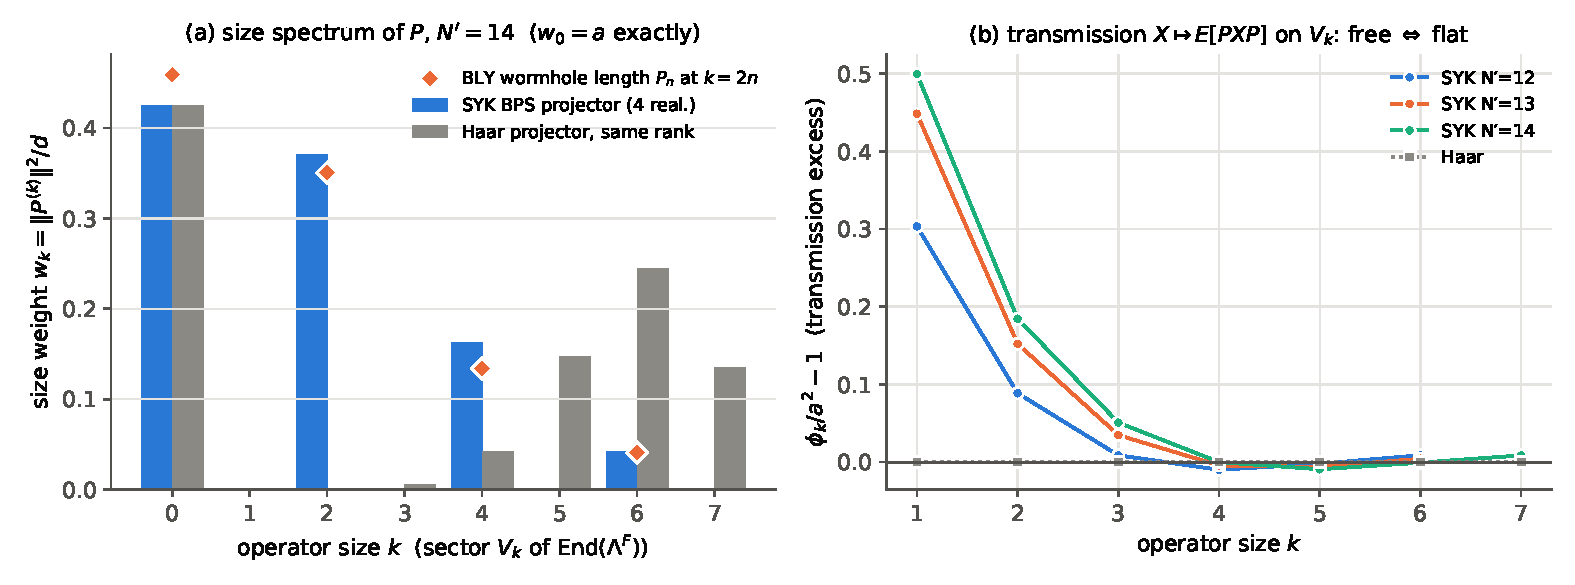
\includegraphics[width=\textwidth]{progress_2026-09-29_figs/fig_size_transmission.pdf}
\caption{(a) \NUM\ Size spectrum of the BPS projector at $\Np=14$. SYK puts its non-identity weight on small, even sizes;
a Haar projector spreads it $\propto\dim V_k$. Orange diamonds: BLY's wormhole-length distribution $P_n$ at
$\lambda=18/14$, placed at $k=2n$ (empirical identification, \S\ref{sec:chordcomp}). (b) \VER\ Transmission excess
$\phi_k/a^2-1$ (\S\ref{sec:transmission}). Haar is flat (0). SYK transmits small operators more than freeness allows,
increasingly with $\Np$, with a small compensating deficit at intermediate $k$ (sum rule~\eqref{eq:phisum}).}
\label{fig:size}
\end{figure}

\subsection{Comparison with the super-chord theory \NUM\ + \INTERP}\label{sec:chordcomp}
Equation~\eqref{eq:rsize} and BLY's $r=\sum_nP_nx^{2n}$ have the same structure. Table~\ref{tab:chordcomp} compares the
ingredients term by term at $k=2n$.
\begin{table}[h]
\centering\small
\begin{tabular}{@{}cc cc cc@{}}
\toprule
$\Np$ & $n$ & $w_{2n}$ (exact size weight) & $P_n$ (BLY, $\lambda=18/\Np$) & $\hat\chi_{2n}(U)$ (exact) & $x^{2n}$ ($x=e^{-2p/\Np}$)\\
\midrule
12 & 0 & 0.5260 & 0.5587 & 1 & 1\\
12 & 1 & 0.3486 & 0.3209 & 0.4359 & 0.3679\\
12 & 2 & 0.1119 & 0.0922 & 0.0769 & 0.1353\\
12 & 3 & 0.0135 & 0.0218 & $-0.0769$ & 0.0498\\
\midrule
14 & 0 & 0.4248 & 0.4588 & 1 & 1\\
14 & 1 & 0.3706 & 0.3506 & 0.5048 & 0.4244\\
14 & 2 & 0.1629 & 0.1339 & 0.1619 & 0.1801\\
14 & 3 & 0.0416 & 0.0407 & $-0.0286$ & 0.0764\\
\bottomrule
\end{tabular}
\caption{\NUM\ The exact size spectrum tracks the chord-length distribution, and the exact characters track the
double-scaled matter weights, each to 10--20\,\%. The sums agree to about 2\,\%, which is consistent with partial
cancellation of the termwise differences.}
\label{tab:chordcomp}
\end{table}

\INTERP\ This is the exact finite-$N$ content of yesterday's wormhole identity:
\begin{itemize}\itemsep1pt
\item the zero-length wormhole $\leftrightarrow$ the identity component $P^{(0)}=a\one$ (weight $w_0=a$ exactly, so the
  $a_\lambda$-vs-$a$ discrepancy disappears);
\item a wormhole of $n$ chords $\leftrightarrow$ the size-$2n$ component;
\item the matter propagator $x^{2n}$ $\leftrightarrow$ the normalized character of the probe on that sector.
\end{itemize}
The pairing $n\leftrightarrow k/2$ is an empirical match, not a derivation (\S\ref{sec:open}).

%=====================================================================
\section{Transmission, and why two BPS spaces are not free}\label{sec:transmission}
%=====================================================================
\subsection{The transmission spectrum \DER}
Define $\Phi(X)=E[PXP]$. By invariance, $\Phi$ commutes with $\Ad_g$ on $\End(\Lambda^F)$, so by Schur it acts on each
$V_k$ as a scalar,
\begin{equation}
\Phi\big|_{V_k}=\phi_k,\qquad E\,\Tr(PXPX^\dagger)=\sum_k\phi_k\,\|X^{(k)}\|^2 \quad\text{for any }X .
\end{equation}
$\phi_k$ is the \emph{transmission} of a size-$k$ operator through the BPS projection. For two independent models,
$E\,\Tr(P_1P_2P_1P_2)=E\,\Tr\big(P_1\Phi(P_1)\big)$, so
\begin{equation}
\boxed{\;E\,\tau(P_1P_2P_1P_2)=\sum_k\phi_k\,w_k\;}
\label{eq:twomodel}
\end{equation}

\subsection{Transmission is a universal function of size \VER}
The superoperator $X\mapsto PXP$, i.e.\ $P\otimes P^T$, is a \emph{realignment} of $|P\rangle\rangle\langle\langle P|$,
the object whose twirl gives $w_k$. Realignment is $U(N)$-equivariant, so it maps the commutant $\mathrm{span}\{\Pi_k\}$
to itself. Hence, per realization (for the $U(N)$-twirled transmissions),
\begin{equation}
\phi_j=\sum_k\mathcal A_{jk}\,\frac{d\,w_k}{\dim V_k},
\end{equation}
with a universal matrix $\mathcal A(N,F)$. We compute $\mathcal A$ on the maximal torus, where the size-$k$ part of a
diagonal operator is its projection onto the $k$-th eigenspace of the Johnson scheme $J(N,F)$ (Appendix~\ref{app:A}).
Verified: brute-force projection of the $400\times400$ superoperator at $N=6$ agrees to $10^{-9}$.

\subsection{Exact sum rules; freeness is flat transmission \VER}
\begin{equation}
\phi_0=a,\qquad \sum_k\phi_k\dim V_k=d^2,\qquad r\big|_{\text{half filling, orbit-averaged}}=\frac{\phi_1}{a}
\label{eq:phisum}
\end{equation}
All three hold per realization to $\le5\times10^{-13}$ for $\Np=8$--14. The third uses the fact that $U=1-2n_i$ has
sizes 0 and 1 only, and it agrees with \eqref{eq:rsize}: two independent exact routes to the orbit-averaged variance.
\begin{itemize}\itemsep1pt
\item \textbf{Haar.} $\phi_{k\ge1}=a(aD^2-1)/(D^2-1)=a^2+O(D^{-2})$ is flat, and \eqref{eq:twomodel} gives
  $2a^2-a^3$, the free value.
\item \textbf{SYK.} The transmission excess $\delta\phi_k=\phi_k-a^2$ is positive at small $k$ (Fig.~\ref{fig:size}b;
  $\delta\phi_1/a^2=+50\%$ at $\Np=14$). By the second sum rule, the dimension-weighted mean of $\delta\phi$ is
  essentially zero.
\end{itemize}
Since $\phi_0=w_0=a$,
\begin{equation}
E\,\tau(P_1P_2P_1P_2)=(2a^2-a^3)+\sum_{k\ge1}\delta\phi_k\,w_k .
\end{equation}
\textbf{Freeness of two BPS spaces is exactly the statement $\delta\phi\equiv0$.} SYK violates it because its size
spectrum and its transmission excess sit at the same small sizes.

\subsection{Two independent SYK models: prediction vs measurement \NUM}
\begin{table}[h]
\centering\small
\begin{tabular}{@{}cccccc@{}}
\toprule
$\Np$ & predicted (from $w_k$) & measured (pairs) & pred./free & meas./free & pairs\\
\midrule
10 & 0.56399 & $0.56406\pm0.00014$ & 1.0056 & 1.0057 & 16\\
12 & 0.41606 & $0.41613\pm0.00149$ (plain) & 1.0203 & 1.0205 & 4\\
 & & $0.41674\pm0.00030$ (c.v.) & & 1.0219 & \\
13 & 0.29481 & -- & 1.0370 & -- & --\\
14 & 0.29661 & $0.29664\pm0.00014$ & 1.0434 & 1.0435 & 16\\
\midrule
Haar & $2a^2-a^3$ & agrees & 1.0000 & 1.000 & 1 per $\Np$\\
\bottomrule
\end{tabular}
\caption{\NUM\ Fourth moment of the principal-angle law between two independent SYK BPS spaces ($\nu$ = squared
cosines of the principal angles). At $\Np=10,14$ the measured value uses a control variate on $\nu-a$, whose expectation
is exactly zero. At $\Np=12$ (only 4 pairs) both the plain mean and the control-variate mean are shown. The latter is
$0.16\%$ ($2\sigma$) above the prediction, and its regression coefficient is poorly determined with 4 pairs. Elsewhere
the parameter-free prediction agrees to $\le0.02\%$. The prediction uses independent seeds (0--3) from the pairs.}
\label{tab:twomodel}
\end{table}

%=====================================================================
\section{The decoder's fourth moment}\label{sec:T4}
%=====================================================================
\subsection{Exact decomposition \VER}
Write $P'=a\one+Y$ with $Y=U(P-a)U$, the rotated nonzero-size part (the reflection fixes the identity component).
With $P^2=P$,
\begin{equation}
T_4=\tau(PP'PP')=\underbrace{a^2}_{\text{no }P'\text{ nontrivial}}+\underbrace{2a\,(T_2-a)}_{\text{one}}+\underbrace{Q_4}_{\text{both}},\qquad Q_4=\frac{\Tr(PYPY)}{d}.
\end{equation}
Splitting $X\mapsto PXP$ into its $U(N)$ twirl (the $\phi_k$) and a remainder $\delta\mathcal P$,
\begin{equation}
Q_4=S+R,\qquad S=\sum_{k\ge1}\phi_kw_k,\qquad R=\frac{\langle Y,\delta\mathcal P\,Y\rangle}{d}.
\end{equation}
\begin{itemize}\itemsep1pt
\item This is exact per realization and for any probe $U$.
\item Free (Haar): $T_2=a$, $S=a^2(1-a)$, $R=0$, so $T_4=2a^2-a^3$. Note that the free $T_4$ already contains
  $a^2(1-a)$ from nonzero sizes; this is the correction to yesterday's conjecture (item 9 of the summary).
\item $R(\one)=(1-a)^2-S$. For a Haar-random probe $g\in U(N)$, $E_gR=0$ and $E_gT_2=a$.
\end{itemize}
Figure~\ref{fig:decomp} shows the three terms as chord pictures.

\begin{figure}[t]
\centering
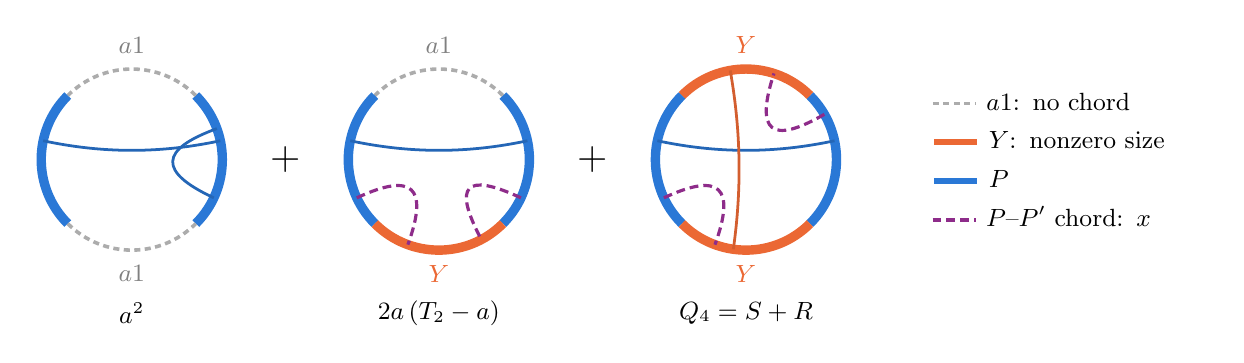
\begin{tikzpicture}
\def\R{1.15}
\begin{scope}
  \draw[Parc] (-45:\R) arc[start angle=-45, end angle=45, radius=\R];
  \draw[triv] (45:\R) arc[start angle=45, end angle=135, radius=\R];
  \draw[Parc] (135:\R) arc[start angle=135, end angle=225, radius=\R];
  \draw[triv] (225:\R) arc[start angle=225, end angle=315, radius=\R];
  \chord[chP]{12}{168}{\R}
  \chord[chP]{-25}{20}{\R}
  \node[gray] at (90:\R+0.3) {\small $a\one$}; \node[gray] at (270:\R+0.3) {\small $a\one$};
  \node[font=\small] at (0,-1.95) {$a^2$};
\end{scope}
\node at (1.95,0) {\Large $+$};
\begin{scope}[xshift=3.9cm]
  \draw[Parc] (-45:\R) arc[start angle=-45, end angle=45, radius=\R];
  \draw[triv] (45:\R) arc[start angle=45, end angle=135, radius=\R];
  \draw[Parc] (135:\R) arc[start angle=135, end angle=225, radius=\R];
  \draw[Pparc] (225:\R) arc[start angle=225, end angle=315, radius=\R];
  \chord[chP]{12}{168}{\R}
  \chord[chX]{205}{250}{\R}
  \chord[chX]{-25}{-62}{\R}
  \node[gray] at (90:\R+0.3) {\small $a\one$}; \node[cPp] at (270:\R+0.3) {\small $Y$};
  \node[font=\small] at (0,-1.95) {$2a\,(T_2-a)$};
\end{scope}
\node at (5.85,0) {\Large $+$};
\begin{scope}[xshift=7.8cm]
  \draw[Parc] (-45:\R) arc[start angle=-45, end angle=45, radius=\R];
  \draw[Pparc] (45:\R) arc[start angle=45, end angle=135, radius=\R];
  \draw[Parc] (135:\R) arc[start angle=135, end angle=225, radius=\R];
  \draw[Pparc] (225:\R) arc[start angle=225, end angle=315, radius=\R];
  \chord[chP]{12}{168}{\R}
  \chord[chPp]{100}{262}{\R}
  \chord[chX]{30}{72}{\R}
  \chord[chX]{205}{250}{\R}
  \node[cPp] at (90:\R+0.3) {\small $Y$}; \node[cPp] at (270:\R+0.3) {\small $Y$};
  \node[font=\small] at (0,-1.95) {$Q_4=S+R$};
\end{scope}
\begin{scope}[xshift=11.9cm]
  \node[align=left, font=\small, text width=3.5cm] at (0,0) {
  \tikz[baseline=-0.6ex]\draw[triv](0,0)--(0.55,0);~$a\one$: no chord\\[3pt]
  \tikz[baseline=-0.6ex]\draw[Pparc,line width=2.2pt](0,0)--(0.55,0);~$Y$: nonzero size\\[3pt]
  \tikz[baseline=-0.6ex]\draw[Parc,line width=2.2pt](0,0)--(0.55,0);~$P$\\[3pt]
  \tikz[baseline=-0.6ex]\draw[chX](0,0)--(0.55,0);~$P$--$P'$ chord: $x$};
\end{scope}
\end{tikzpicture}
\caption{\VER\ + \INTERP\ Exact decomposition of the decoder's fourth moment $T_4=\tau(PP'PP')$ by how many
$P'$-arcs carry nonzero size. Write $P'=a\one+Y$ on each $P'$-arc. The identity part (dashed grey) is the zero-length
wormhole: no chord attaches to it. $Y$ (solid orange) is the nonzero-size part. The first two terms are fixed exactly
by $a$ and the variance. The third splits into $S$, the twirled (``independent-like'') part, exact from the size
spectrum $w_k$, and a genuinely four-point remainder $R$, the correlation between $Y$ and $P$ beyond the twirl.}
\label{fig:decomp}
\end{figure}

\subsection{SYK numbers \NUM}
\begin{table}[h]
\centering\small
\begin{tabular}{@{}ccccccccc@{}}
\toprule
$\Np$ & $a$ & $T_2$ & $T_4$ & $T_4/T_4^{\rm free}$ & $2a(T_2-T_2^{\rm free})$ & $S-Q_4^{\rm free}$ & $R$ & shares of excess\\
\midrule
12 & 0.526 & 0.689 & 0.5994 & 1.470 & $+0.1715$ & $+0.0083$ & $+0.0119$ & 89\,\% / 4\,\% / 6\,\%\\
13 & 0.425 & 0.615 & 0.5063 & 1.750 & $+0.1587$ & $+0.0084$ & $+0.0500$ & 73\,\% / 4\,\% / 23\,\%\\
14 & 0.425 & 0.642 & 0.5342 & 1.879 & $+0.1845$ & $+0.0123$ & $+0.0531$ & 74\,\% / 5\,\% / 21\,\%\\
\midrule
Haar & & $\approx a$ & & $1.000\pm0.001$ & $\approx0$ & 0 & $\approx0$ & --\\
\bottomrule
\end{tabular}
\caption{\NUM\ Decoder fourth moment: mean over 4 realizations $\times$ 5--6 modes. Free baseline: Wachter$(a,b)$
moments of $\mu$ ($T_2^{\rm free}=a$, $Q_4^{\rm free}=a^2(1-a)$ at even $\Np$). The shares add the three pieces of
$T_4-T_4^{\rm free}$. Not shown: $\Np=8,10$ (2 realizations), where $a>0.618$ makes $R(\one)<0$. There $R$ is
negative and the variance term alone exceeds the total excess.}
\label{tab:T4}
\end{table}

\begin{figure}[t]
\centering
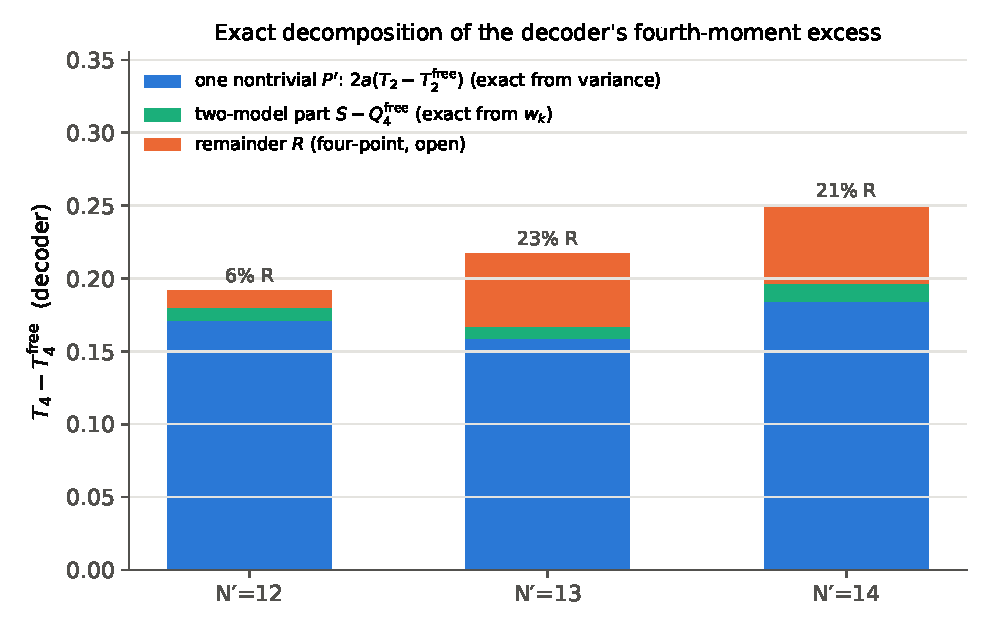
\includegraphics[width=0.68\textwidth]{progress_2026-09-29_figs/fig_T4_decomposition.pdf}
\caption{\NUM\ The decoder's fourth-moment excess over free, split exactly: the variance term (blue), the two-model
size-spectrum term (green) and the four-point remainder $R$ (orange). About 77--79\,\% at $\Np=13$--14 (94\,\% at
$\Np=12$) is fixed exactly by the size spectrum and the variance.}
\label{fig:T4}
\end{figure}

\subsection{What is known about $R$}
\begin{itemize}\itemsep1pt
\item \DER\ The exact limits are $R(\one)=(1-a)^2-S$ and $E_{g\in U(N)}R=0$. $R$ is the only piece that needs
  information beyond the size spectrum: as a class function of the probe, it involves four-copy moments of the
  ensemble.
\item \NUM\ Two natural closures fail.
  \begin{itemize}\itemsep1pt
  \item Size-diagonal characters, $R\approx\sum_{k,k'}\hat\chi_k\hat\chi_{k'}\langle P^{(k)},\delta\mathcal PP^{(k')}\rangle/d$,
    replace the reflection's character on each two-copy irrep in $V_k\otimes V_{k'}$ by its average. This has the
    right sign at $\Np=10,12$ but is 2--5$\times$ too small (0.0055 vs 0.0117 at $\Np=12$).
  \item A ``coherent mixture'' $Y\approx\eta P_{\ge1}+\sqrt{1-\eta^2}\,Y_{\rm indep}$, with $\eta=(T_2-a)/(1-a)$,
    predicts $R=\eta^2R(\one)$, i.e.\ $T_4\approx T_2^2+(1-\eta^2)S$. It is good at $\Np=12$ (mean $-0.3\%$) but
    systematically $4$--$5\%$ low at $\Np=13,14$.
  \end{itemize}
\item \NUM\ Empirically $R/R(\one)=0.23$--$0.25$ at $\Np=13$--14. This lies between $\eta^2\approx0.11$--$0.14$ (the
  mixture ansatz) and $\eta\approx0.33$--$0.38$. $R$ is thus more strongly correlated with the variance than an
  independent-noise ansatz allows. This is an observation, not a law: the single-site probes cluster at few values
  of $\eta$.
\end{itemize}

%=====================================================================
\section{Toward a gravity dual of the decoder}\label{sec:gravity}
%=====================================================================
\subsection{Kinematics versus dynamics}
Every exact identity in \S\S\ref{sec:size}--\ref{sec:T4} follows from $U(N)$ invariance and representation theory. They
hold for \emph{any} $U(N)$-invariant ensemble of projectors. The model-specific content, which is what a gravity dual
must supply, is concentrated in a few spectra:
\begin{enumerate}\itemsep1pt
\item the size spectrum $w_k$ of the BPS projector, which fixes the variance exactly, eq.~\eqref{eq:rsize};
\item nothing more for the two-model fourth moment, since $\phi_k$ is a universal function of $w_k$,
  eq.~\eqref{eq:twomodel};
\item four-copy data for the decoder's remainder $R$.
\end{enumerate}
This sharpens the target. \emph{A gravity dual of the decoder must, first of all, predict the operator-size spectrum of
the BPS projector.} The super-chord theory does so approximately: $w_{2n}\approx P_n$ (Table~\ref{tab:chordcomp}). SYK
serves as the exemplar against which such predictions are tested.

\subsection{Dictionary so far}
Table~\ref{tab:dictionary} collects the correspondences between exact finite-$N$ objects and chord quantities. The
status column separates exact statements from empirical matches.
\begin{table}[h]
\centering\small
\begin{tabular}{@{}>{\raggedright\arraybackslash}p{0.33\textwidth}>{\raggedright\arraybackslash}p{0.35\textwidth}>{\raggedright\arraybackslash}p{0.25\textwidth}@{}}
\toprule
exact finite-$N$ object & chord / gravity counterpart & status\\
\midrule
identity component $P^{(0)}=a\one$, $w_0=a$ & zero-length SUSY wormhole, $P_0$ & exact both; $a_\lambda\neq a$ at $p=3$\\
size spectrum $w_{2n}$ & wormhole-length distribution $P_n$ & empirical, 10--20\,\%\\
character $\hat\chi_k$ of the probe & matter propagator $x^{2n}=q^{2\Delta n}$ & structural analogy\\
$r=a+\sum_{k\ge1}w_k\hat\chi_k$ & $r=\sum_nP_nx^{2n}$ (BLY 4.5--4.8) & exact / 2\,\%\\
transmission $\phi_k$ & zero-$T$ two-point of matter with $\Delta_k=k/p$ & $k\le2$ close at $\Np=12$; $k\ge3$ deviates\\
$P$- and $P'$-arcs; mixed chords cost $x$ & two supercharges, correlation $x$ per chord & exact per chord\\
$\sum_k\delta\phi_kw_k>0$ (two models) & crossings between two chord families & exact / \INTERP\\
decoder $R$ (both $P'$ nontrivial) & four-arc diagrams with mixed chords & open\\
freeness & flat transmission, $x=0$ & exact characterization\\
\bottomrule
\end{tabular}
\caption{Correspondences established or suggested so far.}
\label{tab:dictionary}
\end{table}

\subsection{Next computations}
\begin{enumerate}\itemsep1pt
\item \textbf{Derive $n\leftrightarrow k/2$.} Relate super-chord number to operator size, using the operator-size
  content of BLY's $n_O,n_X$ (their \S5.2, eqs.~5.20--5.23). A derivation would promote Table~\ref{tab:chordcomp}
  from a match to a dictionary entry.
\item \textbf{The four-arc chord computation.} Build the correlated two-supercharge chord Hilbert space: BLY's \S5
  machinery with a Z$_2$ flag per chord that records whether it straddles a $U$. Compute $T_4(x)$, then $R(x)$ and the
  two-model crossing term.
\item \textbf{Two-copy content of $R$.} Characters of the reflection on the irreps of $V_k\otimes V_{k'}$ carrying $R$
  (Casimir on superoperators; feasible for $\Np\le12$).
\end{enumerate}

%=====================================================================
\section{Open questions and dubious points}\label{sec:open}
%=====================================================================
Items that did not pass the audit as established facts, or that are known limitations:
\begin{enumerate}\itemsep2pt
\item \CONJ\ \textbf{$n\leftrightarrow k/2$.} The size-$2n$ weights match $P_n$ to 10--20\,\%. It is not derived why
  one super-chord ``pair'' carries size 2 rather than, say, $p$.
\item \CONJ\ \textbf{Why the closures for $R$ fail.} The proposed reason is that $R$'s weight sits on \emph{small}
  two-copy irreps, where the reflection acts almost trivially. This was inferred, not measured.
\item \textbf{Chord factorization at finite $N$.} The Z$_2$ weight is exact per chord, but independence between chords
  is a double-scaled approximation. The effective per-chord weight at our sizes lies between the exact
  ($1-2p/\Np$) and double-scaled ($e^{-2p/\Np}$) values. Inverting $T_2(x_s)$ for $P_n$ gives $P_1>1$ with the
  former; with the latter the intermediate-$s$ prediction is 5--10\,\% high. For $T_2$ the exact sum rule of \S\ref{sec:size}
  bypasses the issue. For a chord computation of $T_4$ it remains.
\item \INTERP\ \textbf{``$x=0$ = independent models = Haar-random probe.''} The exact content is
  $E_g\,T_4(g)=\sum_k\phi_kw_k$ and $E_gT_2=a$ for $g$ Haar in $U(N)$, per realization; the equality with independent
  models holds in expectation. The parity probe at $s=\Np/2$ is close to but slightly more non-free than two
  independent models ($T_4$: 1.056 vs 1.043 at $\Np=14$), consistent with its small nonzero characters.
\item \textbf{Even sizes at half filling:} numerically exact, but the particle--hole derivation is a sketch with signs
  not tracked.
\item \textbf{Odd $\Np$.} The free baseline must use Wachter$(a,b)$ with $b\neq\frac12$ (done here). The mixture ansatz
  and the $R$ analysis have not been generalized.
\item \textbf{Asymptotics.} Everything is at $\Np\le14$ ($\le16$ for $r$). The $x$-independent non-freeness grows with
  $\Np$ (0.6 $\to$ 4.3\,\%), and $R$'s share grows (6 $\to$ 21\,\%). Their large-$\Np$ fate, including the difference
  between double scaling and fixed $p=3$, is unknown.
\item \textbf{Statistics.} $\Np=14$ uses 4 realizations for sizes and $T_4$. The parity-family sum rule holds within
  $2.5\sigma$, with tensions of $+2.4\sigma$ ($\Np=14$, $s=7$) and $-2.0\sigma$ ($\Np=13$, $s=3$).
\item \textbf{The density.} Only moments through $T_6$ are studied. The spectral density itself has not been
  reconstructed or predicted.
\item \textbf{Superseded:} ``the free (Wachter) law is the zero-length truncation of the chord computation.'' This is
  true for $m_2$ only (\S\ref{sec:T4}); the working note's ``falsified in strong form'' is replaced by the exact
  statement above.
\end{enumerate}

\appendix
\section{Derivation details}
\subsection{The reflection's characters}\label{app:reflection}
Averaging $U_v=1-2n_v$ over its $U(N)$ orbit means $n_v=\sum_{ab}v_a\bar v_bE_{ab}$ with $v$ a Haar-random unit vector.
Haar moments give $E_v[n_v]=\hat N/N=F/N$ and
\[
E_v[n_vXn_v]=\frac{\hat NX\hat N+\sum_{ab}E_{ab}XE_{ba}}{N(N+1)} .
\]
Write $\sum_{ab}E_{ab}XE_{ba}=c_FX-\frac12C(X)$, with $c_F=\sum_{ab}E_{ab}E_{ba}|_{\Lambda^F}=F(N+1-F)$ (checked
numerically). Then
\[
E_v[U_vXU_v]=X\Big[1-\frac{4F}{N}+\frac{4(F^2+c_F)}{N(N+1)}\Big]-\frac{2}{N(N+1)}C(X)=X-\frac{2}{N(N+1)}C(X).
\]
On $V_k$, $C=2k(N+1-k)$, which gives $\hat\chi_k(U)=1-4k(N+1-k)/(N(N+1))$. Checked against the Krawtchouk form to
$10^{-16}$ for $N=7\ldots20$.

\subsection{The transmission matrix}\label{app:A}
$\Tr[\mathcal R(Y)\Ad_g]=\langle\langle\rho(g)^\dagger|Y|\rho(g)^\dagger\rangle\rangle$. So column $k$ of $\mathcal A$ is
the character expansion of the class function $g\mapsto\|\rho(g)^{(k)}\|^2$. On the torus $\rho(g)=\mathrm{diag}(z^S)$,
and its size-$k$ part is the projection onto the $k$-th Johnson eigenspace ($S_N$ irrep $(N-k,k)$, the weight-zero
space of $V_k$), with entries $e_k(r)$ depending on $r=|S\setminus T|$. Using
$\sum_{|S\setminus T|=r}z^S\bar z^T=\binom{N-2r}{F-r}m_r$ and
$\chi_{V_k}=\sum_r\big[\binom{N-2r}{k-r}-\binom{N-2r}{k-r-1}\big]m_r$ gives a triangular system for each column.

\subsection{Haar transmission}
For Haar $P$ of rank $d$, the Weingarten formula gives $E[PXP]=\frac{d(dD-1)}{D(D^2-1)}X$ on traceless $X$. So
$\phi_{k\ge1}=a(aD^2-1)/(D^2-1)$, and $\sum_k\phi_kw_k=2a^2-a^3+O(D^{-2})$.

\section{Reproducibility}
All numbers are exact linear algebra; every heavy run was under the memory watchdog (peak $\le1.0$\,GB).
\begin{center}\small
\begin{tabular}{@{}>{\raggedright\arraybackslash}p{0.27\textwidth}>{\raggedright\arraybackslash}p{0.68\textwidth}@{}}\toprule
Item & Code / data\\\midrule
Parity family (Fig.~\ref{fig:family}, Tab.~\ref{tab:family}) & \path{scripts/run_parity_family.py}, \path{scripts/analyze_parity_family.py}; \path{results/data/parity_family_2026-09-29/raw_q3_N*.jsonl}, \path{summary.csv}\\
Size spectrum, sum rule (Tab.~\ref{tab:sumrule}, \ref{tab:chordcomp}) & \path{src/size_decomposition.py}, \path{scripts/run_size_decomposition.py}, \path{scripts/analyze_size_sumrule.py}; \path{size_q3_N*.jsonl}\\
Transmission, two models (Fig.~\ref{fig:size}b, Tab.~\ref{tab:twomodel}) & \path{scripts/run_two_model_overlap.py}, \path{scripts/analyze_two_copy.py}; \path{two_model_q3_N*.jsonl}, \path{two_copy_tables.md}\\
Decoder $T_4$ (Tab.~\ref{tab:T4}, Fig.~\ref{fig:T4}) & \path{scripts/run_decoder_T4.py}, \path{scripts/analyze_decoder_T4.py}; \path{decoderT4_q3_N*.jsonl}, \path{decoderT4_tables.md}\\
Figures & \path{scripts/plot_progress_2026-09-29.py} $\to$ \path{results/figures/progress_2026-09-29/}\\
Tests & \path{tests/test_size_decomposition.py} (Casimir spectrum, characters, $w_0=a$, Haar sum rule, brute-force transmissions, exact $T_4$ decomposition)\\
Working note and audit & \path{research/notes/decoder_moments_2026-09-29.md}, \path{research/notes/decoder_moments_audit_2026-09-29.md}\\
\bottomrule
\end{tabular}
\end{center}
\paragraph{Realizations and seeds.} $p=3$, $F=\lfloor\Np/2\rfloor$ throughout.
\begin{itemize}\itemsep1pt
\item SYK coupling seeds 0--3 for the parity family ($\Np=8$--14), the size spectra ($\Np=8$--14) and the decoder
  $T_4$ at $\Np=12$--14. The decoder $T_4$ at $\Np=8,10$ uses seeds 0--1.
\item Independent pairs use seeds $(100,101),\ldots,(106,107)$, plus $(110,111),\ldots,(132,133)$ at $\Np=10,14$.
\item Haar controls: seeds 0--1 (parity family; seed 0 at $\Np=13$), seed 0 (sizes, $T_4$), pair $(200,201)$.
\item Single-site probes: 4--6 modes per realization for $T_4$.
\item Data were generated from commit \texttt{86fa66e} plus the working tree (recorded in \path{meta_*.json}). The
  report is at \texttt{774934a} plus the uncommitted audit, figure script and this file.
\end{itemize}

\begin{thebibliography}{9}\small
\bibitem{CV} J.~Chryssanthacopoulos and D.~Vegh, \emph{Fortuity and fragility in supersymmetric SYK}, arXiv:2608.12160 (2026).
\bibitem{BLY} J.~Boruch, H.~W.~Lin and C.~Yan, \emph{Exploring supersymmetric wormholes in $\mathcal N=2$ SYK with chords}, arXiv:2308.16283 (2023).
\bibitem{LMRS} H.~W.~Lin, J.~Maldacena, L.~Rozenberg and J.~Shan, \emph{Looking at supersymmetric black holes for a very long time}, SciPost Phys.\ \textbf{14} (2023) 128, arXiv:2207.00408.
\bibitem{FGMS} W.~Fu, D.~Gaiotto, J.~Maldacena and S.~Sachdev, \emph{Supersymmetric Sachdev-Ye-Kitaev models}, Phys.\ Rev.\ D \textbf{95} (2017) 026009, arXiv:1610.08917.
\bibitem{NS} A.~Nica and R.~Speicher, \emph{Lectures on the Combinatorics of Free Probability}, London Math.\ Soc.\ Lecture Note Series 335, Cambridge University Press (2006).
\bibitem{CMN} B.~Collins, S.~Matsumoto and J.~Novak, \emph{The Weingarten Calculus}, arXiv:2109.14890 (2021).
\end{thebibliography}

\end{document}
